\documentclass{ximera}

\author{Bart Snapp}

\begin{document}

\textbf{For problems 1--3,} consider the following vectors:
\begin{image}
  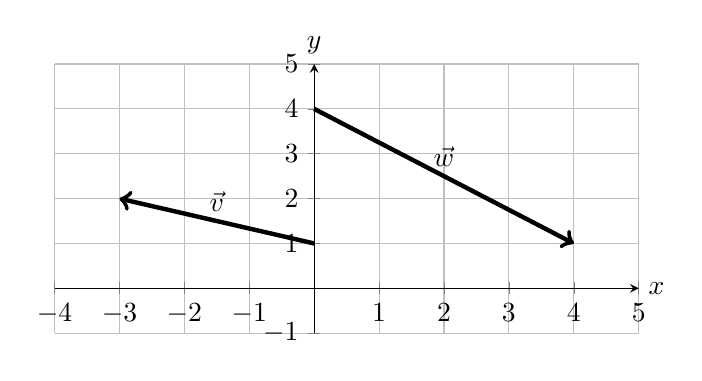
\begin{tikzpicture}[]
    \begin{axis}[
        xmin=-4,xmax=5,ymin=-1,ymax=5,
        clip=false,
        axis lines=center,
        width=9cm,
        height=5cm,
        xtick={-4,-3,...,5},
        ytick={-1,0,...,5},
        xlabel=$x$, ylabel=$y$,
        grid = major,
        every axis y label/.style={at=(current axis.above origin),anchor=south},
        every axis x label/.style={at=(current axis.right of origin),anchor=west},
      ]
      \addplot[ultra thick,black,->] plot coordinates {(0,4) (4,1)};
      \addplot[ultra thick,black,->] plot coordinates {(0,1) (-3,2)};
      \node[above] at (axis cs:2, 2.5) {$\vec{w}$};
      \node[above] at (axis cs:-1.5, 1.5) {$\vec{v}$};
    \end{axis}
  \end{tikzpicture}
\end{image}

\begin{problem}
    \textbf{Draw} $\vec{v}-\vec{w}$ on the grid below.
    \begin{image}
    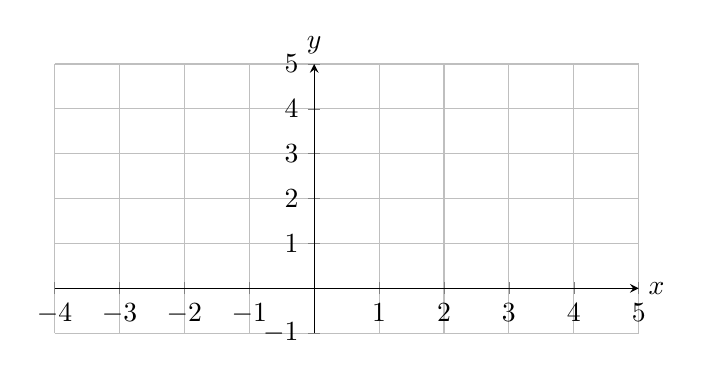
\begin{tikzpicture}[]
    \begin{axis}[
        xmin=-4,xmax=5,ymin=-1,ymax=5,
        clip=false,
        axis lines=center,
        width=9cm,
        height=5cm,
        xtick={-4,-3,...,5},
        ytick={-1,0,...,5},
        xlabel=$x$, ylabel=$y$,
        grid = major,
        every axis y label/.style={at=(current axis.above origin),anchor=south},
        every axis x label/.style={at=(current axis.right of origin),anchor=west},
      ]
      %\addplot[very thick,black,->] plot coordinates {(1,1) (4,2)};
      %\addplot[very thick,black,->] plot coordinates {(-1,0) (-3,3)};
      %\node[above] at (axis cs:2.5, 1.5) {$\vec{w}$};
      %\node[above] at (axis cs:-2, 1.5) {$\vec{v}$};
    \end{axis}
    \end{tikzpicture}
    \end{image}
    \begin{prompt}
      \begin{multipleChoice}
        \choice[correct]{I've drawn this.}
      \end{multipleChoice}
      \begin{feedback}
        \begin{image}
  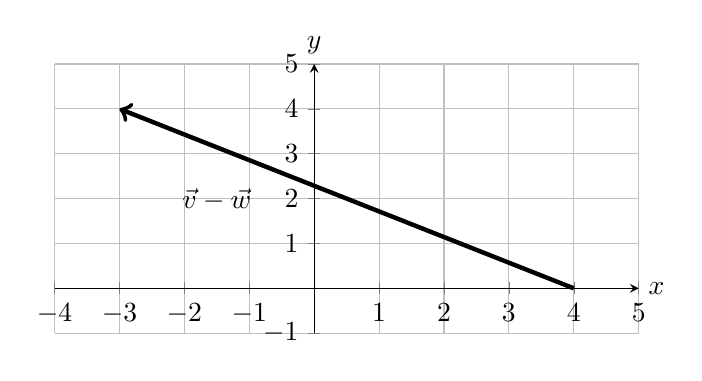
\begin{tikzpicture}[]
    \begin{axis}[
        xmin=-4,xmax=5,ymin=-1,ymax=5,
        clip=false,
        axis lines=center,
        width=9cm,
        height=5cm,
        xtick={-4,-3,...,5},
        ytick={-1,0,...,5},
        xlabel=$x$, ylabel=$y$,
        grid = major,
        every axis y label/.style={at=(current axis.above origin),anchor=south},
        every axis x label/.style={at=(current axis.right of origin),anchor=west},
      ]
      \addplot[ultra thick,black,->] plot coordinates {(4,0) (-3,4)};
      \node[above] at (axis cs:-1.5, 1.5) {$\vec{v}-\vec{w}$};
    \end{axis}
  \end{tikzpicture}
\end{image}
      \end{feedback}
    \end{prompt}
  \end{problem}
  \begin{problem}
    Give a ``calculator-ready'' expression that \textbf{computes the angle}
    between $\vec{v}$ and $\vec{w}$.

    \vfill
    \begin{prompt}
      \[
      \theta = \answer{\arccos(-3/\sqrt{10}}
      \]
    \end{prompt}

  \end{problem}


  \begin{problem}
    Compute the \textbf{area of the parallelogram} spanned by $\vec{v}$ and $\vec{w}$.

    \begin{prompt}
      \[
      \text{Area} = \answer{5}
      \]
    \end{prompt}

    \vfill
  \end{problem}

\end{document}
